\documentclass[xcolor=table]{beamer}

\makeatletter
\definecolor{beamer@blendedblue}{RGB}{0, 145, 95} % changed this
\definecolor{dkblue}{rgb}{0,0.1,0.5}
\definecolor{bluegreen}{rgb}{0,0.5,0.5}
\definecolor{dkgreen}{rgb}{0,0.6,0}
\definecolor{dkred}{rgb}{0.6,0,0}
\definecolor{dkpurple}{rgb}{0.7,0,0.4}
\definecolor{purple}{rgb}{0.7,0,0.7}
\definecolor{olive}{rgb}{0.5, 0.5, 0.0}

\usefonttheme{professionalfonts} % using non standard fonts for beamer
\usepackage{fontspec}
\setmainfont{Gill Sans}
%TIKZ

\usepackage{graphicx}
\usepackage{tikz}
\usepgflibrary{plotmarks}
\usetikzlibrary{calc,shapes.symbols,matrix,shapes.multipart,positioning,fit}
\usetikzlibrary{backgrounds}
\usetikzlibrary{decorations.pathmorphing}
\usetikzlibrary{shapes.callouts}
\usetikzlibrary{shapes.geometric}
\tikzset{snake it/.style={decorate, decoration=snake}}

% Avoid bug with callouts and Beamer, see http://tex.stackexchange.com/questions/31921/callout-and-beamer
\usetikzlibrary{decorations.text}

\usetheme{Execushares}
%for stack drawings
\usepackage{drawstack}
\usepackage{bcprules}
\usepackage{color}
\usepackage{pifont}
\usepackage{amsthm}
\usepackage{thmtools}
\usepackage{caption}
\captionsetup[figure]{labelformat=empty}

% \declaretheorem[numberwithin=chapter]{theorem}
% \declaretheorem[sibling=theorem]{definition}
% \declaretheorem[sibling=theorem]{lemma}

\usepackage{xspace}
\newcommand*{\ii}[1]{\textit{#1}}
\newcommand*{\EG}{e.g.,\xspace}
\newcommand*{\IE}{i.e.,\xspace}
\newcommand*{\ETC}{etc.\xspace}
\newcommand*{\ETAL}{{\em et al.}\xspace}
\newcommand{\atom}[2]{#1@#2}

\newcommand{\mem}[0]{\ii{mem}\xspace}
\newcommand{\imem}[0]{\ii{im}\xspace}
\newcommand{\dmem}[0]{\ii{dm}\xspace}
\newcommand{\reg}[0]{\ii{reg}\xspace}
\newcommand{\ok}[0]{\ii{ok}\xspace}
\newcommand{\astat}[4]{\ensuremath{(#1,#2,#3,#4)}}
\newcommand{\acfistat}[5]{\ensuremath{(#1,#2,#3,#4,#5)}}
\newcommand{\rd}[2]{#1[#2]}
\newcommand{\upd}[3]{#1[#2{\leftarrow}#3]}
\newcommand{\pc}[0]{\ii{pc}\xspace}
\newcommand{\tpc}[0]{t_\ii{pc}}
\newcommand{\tra}[0]{t_\ii{ra}}
\newcommand{\ti}[0]{t_\ii{i}}
\newcommand{\targ}[1]{t_\ii{#1}}
\newcommand{\old}{_{\mathit{old}}}
\newcommand{\extra}[0]{\ii{int}}
\newcommand{\step}[2]{\ensuremath{#1\to#2}}
\newcommand{\stepn}[2]{\ensuremath{#1\to_n#2}}
\newcommand{\stepa}[3]{\ensuremath{#1\to_a^{#3}#2}}


\newcommand{\DATA}[0]{\ii{Data}}
\newcommand{\INSTRname}[0]{\ii{Code}\xspace}
\newcommand{\INSTR}[1]{\INSTRname~#1}
\newcommand{\DATAname}[0]{\ii{Data}\xspace}
\newcommand{\CFG}[0]{$\mathcal{CFG}$\xspace}
\newcommand{\CFGm}[0]{\mathcal{CFG}\xspace}
\newcommand{\SUCC}[1]{$\mathcal{SUCC_\CFGm^{#1}}$\xspace}
\newcommand{\SUCCm}[1]{\mathcal{SUCC_\CFGm^{#1}}\xspace}

\newcommand{\frule}[8]{#1:\{\ifthenelse{\equal{#2}{}}{}{\mathit{PC}{=}#2\ifthenelse{\equal{#3}{}}{}{,}}
                           \ifthenelse{\equal{#3}{}}{}{\mathit{CI}{=}#3}\ifthenelse{\equal{#4}{}}{}{,}
                           \ifthenelse{\equal{#4}{}}{}{\mathit{OP}_1{=}#4}\ifthenelse{\equal{#5}{}}{}{,}
                           \ifthenelse{\equal{#5}{}}{}{\mathit{OP}_2{=}#5}\ifthenelse{\equal{#6}{}}{}{,}
                           \ifthenelse{\equal{#6}{}}{}{\mathit{MR}{=}#6}
                           \} \to \{\mathit{PC}'{=}#7, \mathit{RES}{=}#8\}}

\newcommand{\TAGS}[1]{$\mathcal{T} = \lbrace #1 \rbrace$}

\definecolor{ForestGreen}{RGB}{0, 155, 85}
\definecolor{Purple}{RGB}{153, 71, 155}
\definecolor{BrickRed}{RGB}{182, 50, 28}
\definecolor{darkgreen}{cmyk}{0.7, 0, 1, 0.5}

\begin{document}
\title{Formally Verified Tag-Based Enforcement of Control Flow Integrity}   
\author{Nick Giannarakis} 
\date{\today} 

\pgfdeclarelayer{background}
\pgfdeclarelayer{foreground}
\pgfsetlayers{background,main,foreground}

\frame{\titlepage} 

%1st run : 70sec

\frame{
\frametitle{Motivation}
Modern computers are vulnerable to a wide-range of attacks.
\begin{block}{Common attack technique}
\begin{enumerate}
\item Exploit low-level vulnerability (\EG buffer overflows)
\item Hijack the control-flow of the program to direct execution to
attacker code
\end{enumerate}
\end{block}
%CFG shape with attacker
}

\begin{frame}[fragile]
\frametitle{Defense Mechanisms}
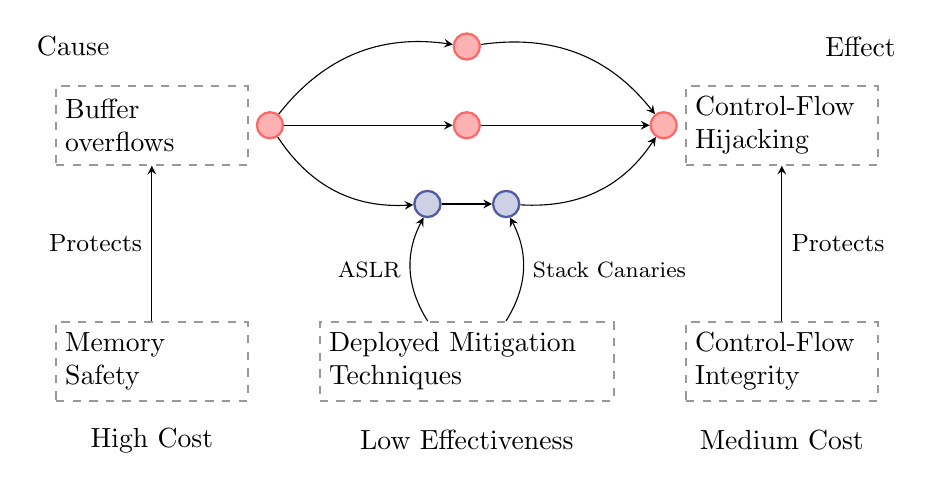
\begin{tikzpicture}
  [attack/.style={rectangle,draw=gray!80,text=black,thick,dashed,minimum height=1cm,text width=2.2cm},
  small_attack/.style={circle,draw,thick,draw=red!60,text=black,fill=red!30},
  mitigation/.style={rectangle,draw=gray!80,text=black,thick,dashed,minimum height=1cm,text width=2.2cm},
  label/.style={rectangle},
  >=stealth]
  \node (buffer_overflow) [attack] at (0,0)  {Buffer\\overflows};
  \node (na1) [small_attack] at (1.5,0)  {};
  \node (na2) [small_attack] at (4,0)  {};
  \node (na3) [small_attack] at (4,1)  {};
  \node (na4) [small_attack] at (3.5,-1)  {};
  \node (na5) [small_attack] at (4.5,-1)  {};
  \node (na6) [small_attack] at (6.5,0)  {};
  \node (cfg_hijack) [attack] at (8,0)  {Control-Flow\\Hijacking};
  
  \path[->]
  (na1) edge [] node {} (na2)
        edge [bend left] node {} (na3)
        edge [bend right] node {} (na4)
  (na2) edge [] node {} (na6)
  (na3) edge [bend left] node {} (na6)
  (na4) edge [] node {} (na5)
  (na5) edge [bend right] node {} (na6);

  %memory safety
  \onslide<2-> 
  { \node (memory_safety) [mitigation] at (0,-3) {Memory Safety};
    \node [rectangle] (high cost) at (0,-4) {High Cost};
    \draw [->]
              (memory_safety)
              to node [left,font=\small] {Protects}
              (buffer_overflow);}

  %deployed mitigation techniques
  \onslide<3->
  { \node (low_level_mitigations) [mitigation,text width=3.5cm] at (4,-3) {Deployed Mitigation\\ Techniques};
    \node [rectangle] (low effectiveness) at (4,-4) {Low Effectiveness};
    \node (na4m) [small_attack,draw=dkblue!70,fill=dkblue!20] at (3.5,-1)  {};
    \node (na5m) [small_attack,draw=dkblue!70,fill=dkblue!20] at (4.5,-1)  {};
    \path[]
    (low_level_mitigations) edge [->,bend left,left,font=\footnotesize] node {ASLR} (na4)
    (low_level_mitigations) edge [->,bend right,right,font=\footnotesize] node {Stack Canaries} (na5);}
  
  %CFI
  \onslide<4->
  { \node (cfi) [mitigation] at (8,-3) {Control-Flow\\Integrity};
    \node [rectangle] (cfi_cost) at (8,-4) {Medium Cost};
    \draw [->]
              (cfi)
              to node [right,font=\small] {Protects}
              (cfg_hijack);}

    
  \node [rectangle] (cause) at (-1,1) {Cause};
  \node [rectangle] (effect) at (9,1) {Effect};
\end{tikzpicture}
\begin{block}{Deployed mitigation techniques}
  \begin{itemize}
    \setlength{\itemsep}{1pt}
  \item Mostly low-level ad-hoc solutions (\EG ASLR, stack canaries, \ETC)
  \item Only make it harder to exploit vulnerabilities
  \item Lack (formal) reasoning about class of attacks thwarted
  \end{itemize}
\end{block}
\end{frame}

%1st run: 53sec
\frame{
\frametitle{Control-Flow Integrity}
Constraints all execution paths to follow a statically computed control-flow graph.
%CFG diagram that kills attacker
\begin{itemize} 
\item Formally provable that CFI defends against attackers who have control over the memory and registers of the machine
\item Effectiveness and efficiency determined by precision of the CFG.
  \begin{itemize}
    \item \textit{Coarse-grained} CFI uses a conservative CFG 
      (\EG instructions are either jump targets or not)
      \begin{itemize}
      \item This approach is vulnerable [G{\"o}tkas \ETAL 2014, 2nd reference]
      \item Most CFI implementations compromise precision for efficiency [Abadi \ETAL 2005, Zhang \ETAL]
    \end{itemize} 
  \end{itemize}
\end{itemize}
}

\frame{
\frametitle{Micro-policies}
\begin{block}{Key Ideas}
  \begin{itemize}
  \small
  \setlength{\itemsep}{0.5pt}
    \item Associate meta-data (tags) to each machine word
    \item Check security invariants and propagate meta-data using to policy-specific set of rules
  \end{itemize}
\end{block}\pause

\begin{block}{Efficient hardware-software implementation}
\begin{itemize}
  \setlength{\itemsep}{0.5pt}
  \small
  \item Hardware propagates the meta-data according to \textbf{software} rules (policy monitor)
    \begin{itemize}
      \item Formally verified micro-policies for memory safety, dynamic sealing,
        compartmentalization and \textbf{CFI} (today's talk)
      \end{itemize}
  \item Hardware rule cache for common-case efficiency
\end{itemize}
\end{block}\pause

\begin{block}{Verification framework}
\begin{itemize}
  \small
  \setlength{\itemsep}{0.5pt}
  \item Models simplified RISC architecture augmented with the above hardware-software mechanism
  \item Intermediate step (Symbolic machine) abstracts away from low-level hardware details
  \item $\lbrace 0,1 \rbrace$-backward simulation between Concrete and Symbolic
\end{itemize}
\end{block}
}

\frame{
\frametitle{CFI Micro-Policy Verification}
\framesubtitle{Proof Structure}
  \begin{center}
    \begin{tikzpicture}
      [machine/.style={rectangle,draw=teal!80,fill=teal!10,text=black,very thick,minimum height=1cm},
       cfi/.style={rectangle,draw,thick,draw=teal!80,text=black,fill=teal!10},
       >=stealth]

      % abstract
      \onslide<3->{\node [machine,fill=teal!10] (abstract) {CFI Abstract Machine};}

      % symbolic-rule
      \node (symbolic label) [below=2.5cm of abstract] {Symbolic Machine};
      \node [rectangle,draw,thick,fill=teal!20,rounded corners]
            (symbolic rules) [right=of symbolic label] {CFI Micro-Policy};
      \begin{pgfonlayer}{background}
        \node [machine,dashed,fill=teal!10,fit={(symbolic label) (symbolic rules)}]
              (symbolic) {};
      \end{pgfonlayer}
      \onslide<5->{\node [cfi,right=of symbolic] (symbolic cfi) {CFI Property};}

      %abstract cfi
      \onslide<4->
      {\node [cfi] (abstract cfi)  at (abstract -| symbolic cfi) {CFI Property};
       \draw [thick] (abstract) to (abstract cfi);}

      %symbolic cfi
      \onslide<5->{
        \draw [thick] (symbolic) to (symbolic cfi);
        \draw [->,thick]
              (abstract cfi)
              to node [right,text width=2cm,font=\footnotesize] {Preserved\\by backward\\
                simulation}
              (symbolic cfi);}

      % concrete
      \onslide<2->{\node (concrete label) [below=2.5cm of symbolic label] {Concrete
        Machine};
      \node [rectangle,draw,thick,fill=gray!20,rounded corners]
            (fault handler) [right=of concrete label] {CFI Policy Monitor};
      \begin{pgfonlayer}{background}
        \onslide<2->{
        \node [machine,dashed,fill=teal!10,fit={(concrete label) (fault handler)}]
              (concrete) {};}
      \end{pgfonlayer}}
      % \draw [thick,dashed] (concrete) to (concrete cfi);
      \onslide<6->{\node [cfi] (concrete cfi) at (concrete -| symbolic cfi) {CFI Property};}


      \onslide<2->{\draw [color=gray!70,thick,->]
        (symbolic rules.center |- symbolic rules.south)
        -- node [right] {Compiled to}
        (symbolic rules.center |- fault handler.north);}

      \onslide<2->{\draw [<->,thick,dashed]
            (abstract.center |- symbolic.south)
            -- node [left] {Simulates}
            (abstract.center |- concrete.north);}

      \onslide<3->{\draw [<->,thick]
            (abstract)
            -- node [left] {Simulates}
            (abstract.center |- symbolic.north);}

       \onslide<6-> {
         \node [color=ForestGreen,scale=1.4] (success) [right=0.1cm of concrete cfi] {\ding{51}};
         \draw [thick] (concrete) to (concrete cfi);
         \draw [->,thick]
              (symbolic cfi)
              to[] node [right,text width=2cm,font=\footnotesize] {Preserved\\by backward\\
                simulation}
              (concrete cfi);}
    \end{tikzpicture}
  \end{center}
}

\frame{
  \frametitle{CFI Micro-Policy Verification}
  \framesubtitle{Proof Structure Advantages}
  This proof organization offers significant advantages
  \begin{itemize}
    \item We avoided a complex direct proof of the CFI property
      on the Concrete Machine
    \item It reduced proof effort by allowing us to use the simulation between the Concrete and
      the Symbolic Machine that is provided by the Micro-Policies framework
    \item It allowed us to do most of our reasoning on the Symbolic machine, using structured
      mathematical objects instead of bits
    \item The reusable nature of the preservation theorem allowed us to introduce one more
      level of abstraction (Abstract Machine)
    \item The refinement between the Concrete Machine and the correct by construction
      machine provides additional assurance in the correctness of the micro-policy
    \end{itemize}
}

\frame{
\frametitle{CFI Micro-policy}
Formalized micro-policy includes fine-grained CFI, non-writable code (NWC) and non-executable data (NXD)
\begin{block}{Set of tags}
  \TAGS{\DATA,\INSTR{\ii{id}}, \INSTR{\bot}} %write as ADT
\end{block}
\begin{block}{Tagging scheme}
  \begin{itemize}
  \item Non-executable data are tagged \DATA.
  \item Sources/targets of indirect control-flows (according to CFG) are tagged \INSTR{\textit{id}}
    \begin{itemize}
      \item We use the address of the instruction as an \textit{id}
    \end{itemize}
  \item All other instructions are tagged $\INSTR{\bot}$
  \item The \pc is tagged \INSTR{\ii{id}} or \DATA
  \item All other registers are tagged \DATA
  \end{itemize}
\end{block}
}

% make it with pauses. 
\frame{
\frametitle{CFI micro-policy}
\framesubtitle{Example}
\begin{table}[h]
\centering
\small
\begin{tabular}{lllcll}
                          &              &             & r                                                &           &           \\ \cline{2-6} 
\multicolumn{1}{c|}{Regs} & \multicolumn{2}{c|}{$\ldots$} & \multicolumn{1}{c|}{\atom{500}{\DATA}} & \multicolumn{2}{l|}{$\ldots$} \\ \cline{2-6} 
\end{tabular}
\end{table}

\centering
\begin{minipage}[b]{0.42\linewidth}
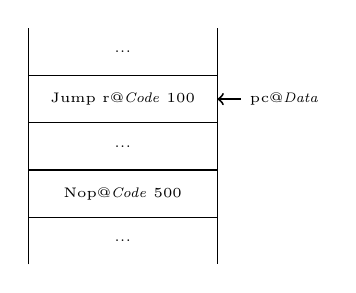
\begin{tikzpicture}[scale=0.6,font=\tiny]
  \small
  \stacktop[]{}
  \cell[]{\atom{Jump r}{\INSTR{100}}} \celladdr{100} \cellptr{\atom{pc}{\DATA}}
  \stackbottom[]{}
  \cell[]{\atom{Nop}{\INSTR{500}}} \celladdr{500}
  \stackbottom[]{}
\end{tikzpicture}
\end{minipage}
\hspace{0.5em}
\begin{minipage}[b]{0.45\linewidth}
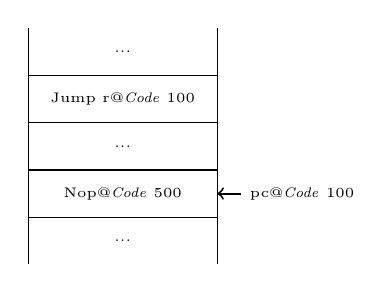
\begin{tikzpicture}[scale=0.6,font=\tiny]
  \small
  \stacktop[]{}
  \cell[]{\atom{Jump r}{\INSTR{100}}} \celladdr{100} 
  \stackbottom[]{}
  \cell[]{\atom{Nop}{\INSTR{500}}} \celladdr{500} \cellptr{\atom{pc}{\INSTR{100}}}
  \stackbottom[]{}
\end{tikzpicture}
\end{minipage}
$(100,500) \in \CFGm$?
}

%Abstract Machine
\frame{
\frametitle{CFI Abstract Machine}
The Abstract Machine acts as a specification for CFI
\begin{itemize}
\setlength{\itemsep}{1pt}
\item Instructions fetched from fixed instruction memory (NWC, NXD)
\item State includes \ok bit as indication of a violation. The machine is stuck if it is set to false.
\end{itemize}
\infrule[Jump]{
  \imem[\pc] = i \andalso \ii{decode}~i = \ii{Jump}~r \\
  \rd{\reg}{r} = \pc' \andalso
  \ii{ok} = (\pc,\pc') \in \CFGm
  }{\step{\acfistat{\imem}{\dmem}{\reg}{\pc}{\ii{true}}}{
    \acfistat{\imem}{\dmem}{\reg}{\pc'}{\ii{ok}}}}
\infrule[Store]{
  \imem[\pc] = i \andalso \ii{decode}~i = \ii{Store}~r_p~r_s \andalso
  \rd{\reg}{r_p} = p \\
  \rd{\reg}{r_s} = w \andalso
  \dmem' = \upd{\dmem}{p}{w}
  }{\step{\acfistat{\imem}{\dmem}{\reg}{\pc}{\ii{true}}}{
    \acfistat{\imem}{\dmem'}{\reg}{\pc+1}{\ii{true}}}}
}

%Symbolic Machine
\begin{frame}[fragile]
\frametitle{CFI Symbolic Machine}

Uses structured mathematical objects (ADTs, functions, \ETC)

\begin{itemize}
\item $type = \DATA ~|~\INSTR{id}~|~\INSTR{\bot}$
  \begin{itemize}
    \item Denotes set of tags
    \end{itemize}
\item $transfer~:~ ivector \rightarrow ovector$
  \begin{itemize}
    \item Denotes set of rules
    \end{itemize}
\end{itemize}

\infrule[Jump]{
  \mem[\pc] = \atom{i}{t_i} \andalso \ii{decode}~i = \ii{Jump}~r \\
  \rd{\reg}{r} = \atom{\pc'}{t_w} \andalso
  \ii{transfer}~(t_{pc},t_i,t_w,-,-) = (t_{pc}',-)
  }{\step{\astat{\mem}{\reg}{\atom{\pc}{t_{pc}}}{int}}
  {\astat{\mem}{\reg}{\atom{\pc'}{t_{pc}'}}{int}} }
\end{frame}

%Concrete Machine
\begin{frame}
\frametitle{CFI Concrete Machine}
\begin{block}{Policy Monitor self-protection mechanism}
\begin{itemize}
\item Uses tags to distinguish between user-level and policy monitor
  \begin{itemize}
    \item \textit{User ut} where $ut \in \mathcal{T}$
    \item \textit{Monitor} for policy-monitor
    \item \textit{Entry ut} for privileged monitor services from user code
    \item We need to provide encoding scheme from tags to machine words
    \end{itemize}
\item \textit{Policy monitor} is a \emph{correct} implementation of the transfer function in machine code
\end{itemize}
\end{block}
\end{frame}

\begin{frame}[fragile]
\frametitle{Attacker Model}
\begin{block}{Intuition}
  \begin{itemize}
  \item Can change all (\textbf{user-level}) data in memory and registers
  \item But \textbf{not} the code or the tags for tagged machines
  \item Concrete attacker cannot tamper with the machine while it is in Monitor mode
  \end{itemize}
\end{block}
\begin{block}{Formally}
  \small
  \infrule{
  \ii{dom}~\dmem = \ii{dom}~\dmem' \andalso
  \ii{dom}~\reg = \ii{dom}~\reg'
}{
  \stepa{\acfistat{\imem}{\dmem}{\reg}{\pc}{\ok}}
  {\acfistat{\imem}{\dmem'}{\reg'}{\pc}{\ok}}
  {A}}
\centering
\begin{minipage}[b]{0.42\linewidth}
  \small
  \infrule[]{
  }{\stepa{\atom{w_1}{\DATA}}{\atom{w_2}{\DATA}}{S}}
\end{minipage}
\hspace{0.5em}
\begin{minipage}[b]{0.45\linewidth}
  \small
  \infrule[]{
  }{\stepa{\atom{w_1}{\INSTR{id}}}{\atom{w_1}{\INSTR{id}}}{S}}
\end{minipage}
\small
\infrule{
  \stepa{\mem}{\mem'}{S} \andalso
  \stepa{\reg}{\reg'}{S}
}{
  \stepa{\astat{\mem}{\reg}{\atom{\pc}{t}}{\extra}{}}
  {\astat{\mem'}{\reg'}{\atom{\pc}{t}}{\extra}{}}
  {S}
}
\end{block}
\end{frame}

\frame{
\frametitle{CFI Property}
\begin{block}{Definition parameterized by:}
  \begin{itemize}
    \item Set of states \textit{S}
    \item \textit{Initial} states predicate
    \item Attacker model
    \item \SUCC{} function on states that determines if the control-flow is allowed
    \item \textit{Stopping} predicate (on execution traces) characterizing execution after a control-flow violation
  \end{itemize}
  $$M=(\textit{S},\textit{initial},\stepn{}{},\stepa{}{}{},\SUCCm{},\textit{stopping})$$
\end{block}
}

\frame{
\frametitle{CFI Property}
\framesubtitle{Definitions}
\begin{definition}[Trace has CFI]\label{traceHasCfi}
  We say that an execution trace $s_0 \to s_1 \to \ldots \to s_n$ {\em has CFI}
  if for all $ i \in [0,n)$ if \stepn{s_i}{s_{i+1}} then
  $(s_i,s_{i+1}) \in$ \SUCC{}.
\end{definition}\pause
\vspace*{0em}
\begin{alertblock}{
More complicated than Abadi \ETAL because our mechanism can only detect a violation after it has happened!}
\end{alertblock}
\vspace*{-1.4em}
\begin{definition}[CFI]\label{cfi}
  A CFI machine M has CFI with respect to the set of allowed indirect jumps \CFG
  if, for any execution starting from initial state $s_0$
  and producing a trace $s_0 \to \ldots \to s_n$, either
  \begin{enumerate}
  \setlength{\itemsep}{1pt}
  \item The whole trace \emph{has CFI} according to
    the above definition, or else
  \item There is some $i$ such that $s_i \to_n s_{i+1}$,
  and $(s_i, s_{i+1}) \not \in$ \SUCC{}, where
  the sub-traces $s_0 \to \ldots \to s_i$ and
  $s_{i+1} \to \ldots \to s_n$ both have CFI
  and the sub-trace $s_{i+1} \to \ldots \to s_n$ is stopping.
  \end{enumerate}
\end{definition}
}

\frame{
\frametitle{CFI Property}
\framesubtitle{Instances of definitions I}
\begin{block}{Abstract Machine}
  \begin{itemize}
    \setlength{\itemsep}{1pt}
    \item $\mathit{initial^A}$ : \ok bit set to true
    \item \SUCC{A} : Extends \CFG with direct control-flows (\EG Nop targets pc+1)
    \item $\mathit{stopping^A}$ : All states in trace are stuck with respect to \stepn{}{}
  \end{itemize}
\end{block}

\begin{block}{Symbolic Machine}
  \begin{itemize}
    \setlength{\itemsep}{1pt}
    \item $\mathit{initial^S}$ : Indirect jumps and their targets tagged according to \CFG (invariant) and tag on PC is \DATA.
    \item \SUCC{S} : Extends \CFG with direct control-flows (\EG Nop targets pc+1)
    \item $\mathit{stopping^S}$ : All states in trace are stuck with respect to \stepn{}{}
  \end{itemize}
\end{block}
}

\frame{
\frametitle{CFI Property}
\framesubtitle{Instances of definitions II}
\begin{block}{Concrete Machine}
  \begin{itemize}
    \setlength{\itemsep}{1pt}
    \item $\mathit{initial^C}$ : Image of a symbolic state $s^S$ such that $s^S \sim s^C$
    \item \SUCC{C} : Extends \CFG with direct-flows, allows all flows involving monitor mode
    \item $\mathit{stopping^C}$ : There is an optional prefix of attacker steps followed by an optional suffix of
      monitor (normal) steps
  \end{itemize}
\begin{center}
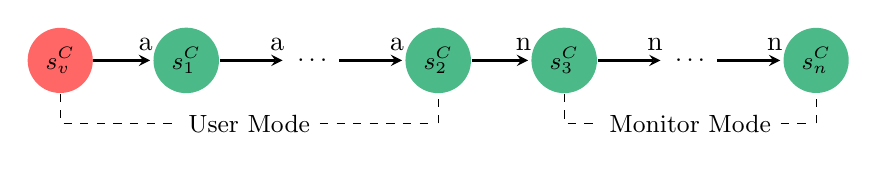
\begin{tikzpicture}
  [scale=.8,auto=left,shorten >=1pt,every node/.style={circle,fill=ForestGreen!70,font=\small},->,>=stealth]
  \node (nv) [style={fill=red!60}] at (0,0)  {$s^C_v$};
  \node (na1) at (2,0)  {$s^C_1$};
  \node (nadots) [draw=none,style={fill=white}] at (4,0)  {$\ldots$};
  \node (na2) at (6,0)  {$s^C_2$};
  \node (nm1) at (8,0)  {$s^C_3$};
  \node (nmdots) [draw=none,style={fill=white}] at (10,0)  {$\ldots$};
  \node (nm2) at (12,0)  {$s^C_n$};

\node (nulabel) [rectangle,fill=white,font=\small] at (3,-1) {User Mode};
\node (na2label) [fill=none] at (6,-1) {};

\node (nmlabel) [rectangle,fill=white,font=\small] at (10,-1) {Monitor Mode};
\node (nm2label) [fill=none] at (12,-1) {};

\draw[-,dashed,very thin] (nv) |- (nulabel);
\draw[-,dashed,very thin] (nulabel.east) |- (na2label.center);
\draw[-,dashed,very thin] (na2label.center) |- (na2.south);

\draw[-,dashed,very thin] (nm1) |- (nmlabel);
\draw[-,dashed,very thin] (nmlabel.east) |- (nm2label.center);
\draw[-,dashed,very thin] (nm2label.center) |- (nm2.south);

\path[thick, every node/.style={}]
(nv) edge [very near end,above] node {a} (na1)
(na1) edge [very near end,above] node {a} (nadots)
(nadots) edge [very near end,above] node {a} (na2)
(na2) edge [very near end,above] node {n} (nm1)
(nm1) edge [very near end,above] node {n} (nmdots)
(nmdots) edge [very near end,above] node {n} (nm2);
\end{tikzpicture} \\
\end{center}
\end{block}
}

\begin{frame}[fragile]
\frametitle{Generic Preservation Theorem}
\framesubtitle{Requirements}
\textbf{Backward simulation preserves CFI}
\begin{itemize}
  \setlength{\itemsep}{0.8pt}
  \item High-level machine $M^H$ related to low-level machine $M^L$ by simulation relation $\sim$
  \item Predicate \textit{checked} on low-level normal steps indicates if step must be checked for CFI 
  \item $\lbrace 0,1 \rbrace$-backward simulation for unchecked steps
  \item 1-backward simulation for checked and attacker steps
\end{itemize}
 \begin{minipage}{\linewidth}
  \centering
  \begin{minipage}{0.45\linewidth}
      \begin{center}
        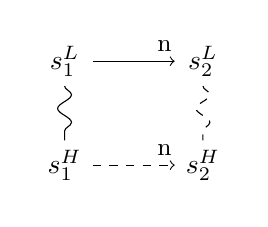
\begin{tikzpicture}
          \matrix (m) [matrix of math nodes,row sep=2em,column sep=3em,minimum width=2em]
          {
            s^L_1 & s^L_2 \\
        s^H_1 & s^H_2 \\};
      \path[->]
      (m-1-1) edge [snake it,-] node {} (m-2-1)
      edge [above] node [above,very near end,font=\small] {n} (m-1-2)
      (m-2-1.east|-m-2-2) edge [dashed, above,very near end,font=\small] node {n}
      node {} (m-2-2)
      (m-1-2) edge [snake it,dashed,-] node {} (m-2-2);
    \end{tikzpicture}
       \end{center}
  \end{minipage}
  \hspace{0.05\linewidth}
  \begin{minipage}{0.45\linewidth}
      \begin{center}
        \begin{tikzpicture}
          \matrix (m) [matrix of math nodes,row sep=2em,column sep=3em,minimum width=2em]
          {
            s^L_0 & s^L_1 \\
            s^H\\};
          \path[->]
          (m-1-1) edge [snake it,-,above] node {} (m-2-1)
          (m-1-1.east|-m-1-2) edge [above,font=\small, very near end] node {n}
          node {} (m-1-2)
          (m-1-2) edge [snake it,dashed,-] node {} (m-2-1);
        \end{tikzpicture}
      \end{center}
  \end{minipage}
  \begin{minipage}{0.45\linewidth}
      \begin{center}
        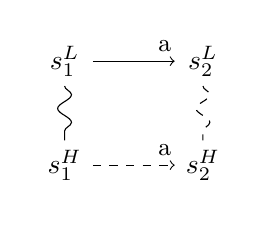
\begin{tikzpicture}
          \matrix (m) [matrix of math nodes,row sep=2em,column sep=3em,minimum width=2em]
          {
            s^L_1 & s^L_2 \\
            s^H_1 & s^H_2 \\};
          \path[->]
          (m-1-1) edge [snake it,-] node {} (m-2-1)
          edge [above] node [above,very near end,font=\small] {a} (m-1-2)
          (m-2-1.east|-m-2-2) edge [dashed, above,very near end,font=\small] node {a}
          node {} (m-2-2)
          (m-1-2) edge [snake it,dashed,-] node {} (m-2-2);
        \end{tikzpicture}
      \end{center}
  \end{minipage}
\end{minipage}
\end{frame}

\frame{
\frametitle{Generic Preservation Theorem}
\framesubtitle{Requirements II}
  Plus some additional assumptions: 
  \begin{itemize}
  \item On initial states, low-level initial states can be mapped to high-level initial states
  \item On the step relation of the low-level machine, we require that it is decidable
  \item On successor functions, for checked steps \SUCC{H} and \SUCC{L} agree on their results
    and for unchecked steps \SUCC{L} allows all steps
  \item On normal steps that are violations, we require that they cannot be attacker steps as well
  \item On stopping traces, a high-level stopping trace is simulated only by a low-level stopping trace
  \end{itemize}
}


\frame{
\frametitle{Using the Preservation Theorem}
\begin{block}{Symbolic-Abstract}
\begin{itemize}
  \item All steps are checked
  \item We have proved 1-backward simulation for normal and attacker steps.
\end{itemize}
\end{block}

\begin{block}{Concrete-Symbolic}
\begin{itemize}
  \item Steps involving the monitor are unchecked
    \begin{itemize}
      \item But by definition of \SUCC{C} they are allowed
      \end{itemize}
  \item We can obtain a $\lbrace 0,1 \rbrace$-backward simulation for normal steps from the framework.
  \item We prove 1-backward simulation for attacker steps.
\end{itemize}
\end{block}
}

%50 sec
\frame{ 
  \frametitle{Conclusions} 
  We formalized and verified, using the
  Coq proof assistant, a dynamic monitor for fine-grained CFI.
  \begin{itemize} 
  \item We provided an attacker model and a proof that all machine
    steps follow the CFG even in the presence of the attacker
  \item We proved a two-way refinement between the concrete machine
    running the CFI dynamic monitor and an abstract machine that has
    CFI by construction
  \end{itemize}
  
  \begin{itemize}
    \item Development: 5799 LOC = 1784 spec + 3800 proof + 215 comments
    \item Part of ``Micro-Policies : A Framework for Verified,
      Hardware-Assisted Security Monitors'' [Azevedo \ETAL, submitted 2014]
    \end{itemize}
}

\frame{
\frametitle{Future Work}
\begin{itemize}
\item Write and verify the machine code for the monitor
  \begin{itemize}
    \item More interesting for more realistic RISC architectures (\EG ARM)
    \item Could also test the code (using QuickChick!) - requires CFG
    \end{itemize}
\item Increase precision by enforcing call-stack protection to ensure correct returns
\end{itemize}
}

%BONUS SLIDES

\section{Bonus Slides}
\frame{
\frametitle{CFI Micro-Policy}
\framesubtitle{Rules}
% \def\beforelabelspacehack{\vspace*{-2ex}}
\small
\infrule[]{
  \ii{op} \in \lbrace \ii{Jump}, \ii{Jal} \rbrace \andalso
  (src,dst) \in \CFGm
  }{
  \ii{op} : \{PC=\INSTR{src},CI=\INSTR{dst}\} \to (\INSTR{dst},-)
  }
\infrule[]{
  \ii{op} \in \lbrace \ii{Jump}, \ii{Jal} \rbrace
  }{
    \ii{op} : \{PC=\DATA,CI=\INSTR{\textit{src}}\} \to (\INSTR{src},-)
  }
\infrule[]{
  (src,dst) \in \CFGm
  }{
  \ii{Store} : \{PC=\INSTR{src},CI=\INSTR{dst},MR=\DATA\} \to (\DATA,\DATA)}
\infrule[]{
  \textit{ti} \in \lbrace \INSTR{dst}, \INSTR{\bot} \rbrace
  }{
  \ii{Store} : \{PC=\DATA,CI=\textit{ti},MR=\DATA\} \to (\DATA,\DATA)
  }
\infrule[]{
  \textit{op} \not \in \lbrace \textit{Jump}, \textit{Jal}, \textit{Store}
  \rbrace \andalso (src,dst) \in \CFGm
  }{
  \textit{op} : \{PC=\INSTR{src},CI=\INSTR{dst}\} \to (\DATA,-)
  }
\infrule[]{
  \textit{op} \not \in \lbrace \textit{Jump}, \textit{Jal}, \textit{Store}
  \rbrace \andalso
  \textit{ti} \in \lbrace \INSTR{dst}, \INSTR{\bot} \rbrace
  }{
  \textit{op} :\{PC=\DATA,CI=\textit{ti}\} \to (\DATA,-)
  }
}

% \begin{frame}[fragile]
% \begin{minipage}{\linewidth}
%   \centering
%   \begin{minipage}{0.45\linewidth}
%     \begin{figure}[H]
%       \begin{center}
%         \begin{tikzpicture}
%           \matrix (m) [matrix of math nodes,row sep=3em,column sep=4em,minimum width=2em]
%           {
%             s^L_1 & s^L_2 \\
%         s^H_1 & s^H_2 \\};
%       \path[->]
%       (m-1-1) edge [snake it,-] node {} (m-2-1)
%       edge [above] node [above,very near end,font=\small] {n} (m-1-2)
%       (m-2-1.east|-m-2-2) edge [dashed, above,very near end,font=\small] node {n}
%       node {} (m-2-2)
%       (m-1-2) edge [snake it,dashed,-] node {} (m-2-2);
%     \end{tikzpicture}
%        \end{center}
%        \caption{1-backward simulation}
%      \end{figure}
%   \end{minipage}
%   \hspace{0.05\linewidth}
%   \begin{minipage}{0.45\linewidth}
%     \begin{figure}[H]
%       \begin{center}
%         \begin{tikzpicture}
%           \matrix (m) [matrix of math nodes,row sep=3em,column sep=4em,minimum width=2em]
%           {
%             s^L_0 & s^L_1 \\
%             s^H\\};
%           \path[->]
%           (m-1-1) edge [snake it,-,above] node {} (m-2-1)
%           (m-1-1.east|-m-1-2) edge [above,font=\small, very near end] node {n}
%           node {} (m-1-2)
%           (m-1-2) edge [snake it,dashed,-] node {} (m-2-1);
%         \end{tikzpicture}
%       \end{center}
%       \caption{0-backward simulation}
%     \end{figure}
%   \end{minipage}
% \hspace{0.05\linewidth}
%   \begin{minipage}{0.45\linewidth}
%     \begin{figure}[H]
%       \begin{center}
%         \begin{tikzpicture}
%           \matrix (m) [matrix of math nodes,row sep=3em,column sep=4em,minimum width=2em]
%           {
%             s^L_1 & s^L_2 \\
%             s^H_1 & s^H_2 \\};
%           \path[->]
%           (m-1-1) edge [snake it,-] node {} (m-2-1)
%           edge [above] node [above,very near end,font=\small] {a} (m-1-2)
%           (m-2-1.east|-m-2-2) edge [dashed, above,very near end,font=\small] node {a}
%           node {} (m-2-2)
%           (m-1-2) edge [snake it,dashed,-] node {} (m-2-2);
%         \end{tikzpicture}
%       \end{center}
%       \caption{1-backward simulation for attacker}
%     \end{figure}
%     \bigskip
%   \end{minipage}
% \end{minipage}
% \end{frame}
\end{document}

